\documentclass[11pt]{article}
\usepackage{graphicx}
\usepackage{amsmath, amssymb, float}
\usepackage{mathtools}
\usepackage{enumitem}
\allowdisplaybreaks

\DeclareMathOperator{\EX}{\mathbb{E}}% expected value
\DeclareMathOperator{\Var}{\operatorname{Var}}% variance
\DeclareMathOperator{\Span}{\operatorname{span}}% span
\DeclareMathOperator{\Ad}{\operatorname{Ad}}% Adjoint
\newcommand{\pd}[2]{\frac{\partial #1}{\partial #2}} % partial derivatives

\title{ROB 530 Project Notes}
\author{rlybrdgs }

\begin{document}

\maketitle

\begin{figure}[H]
    \centering
    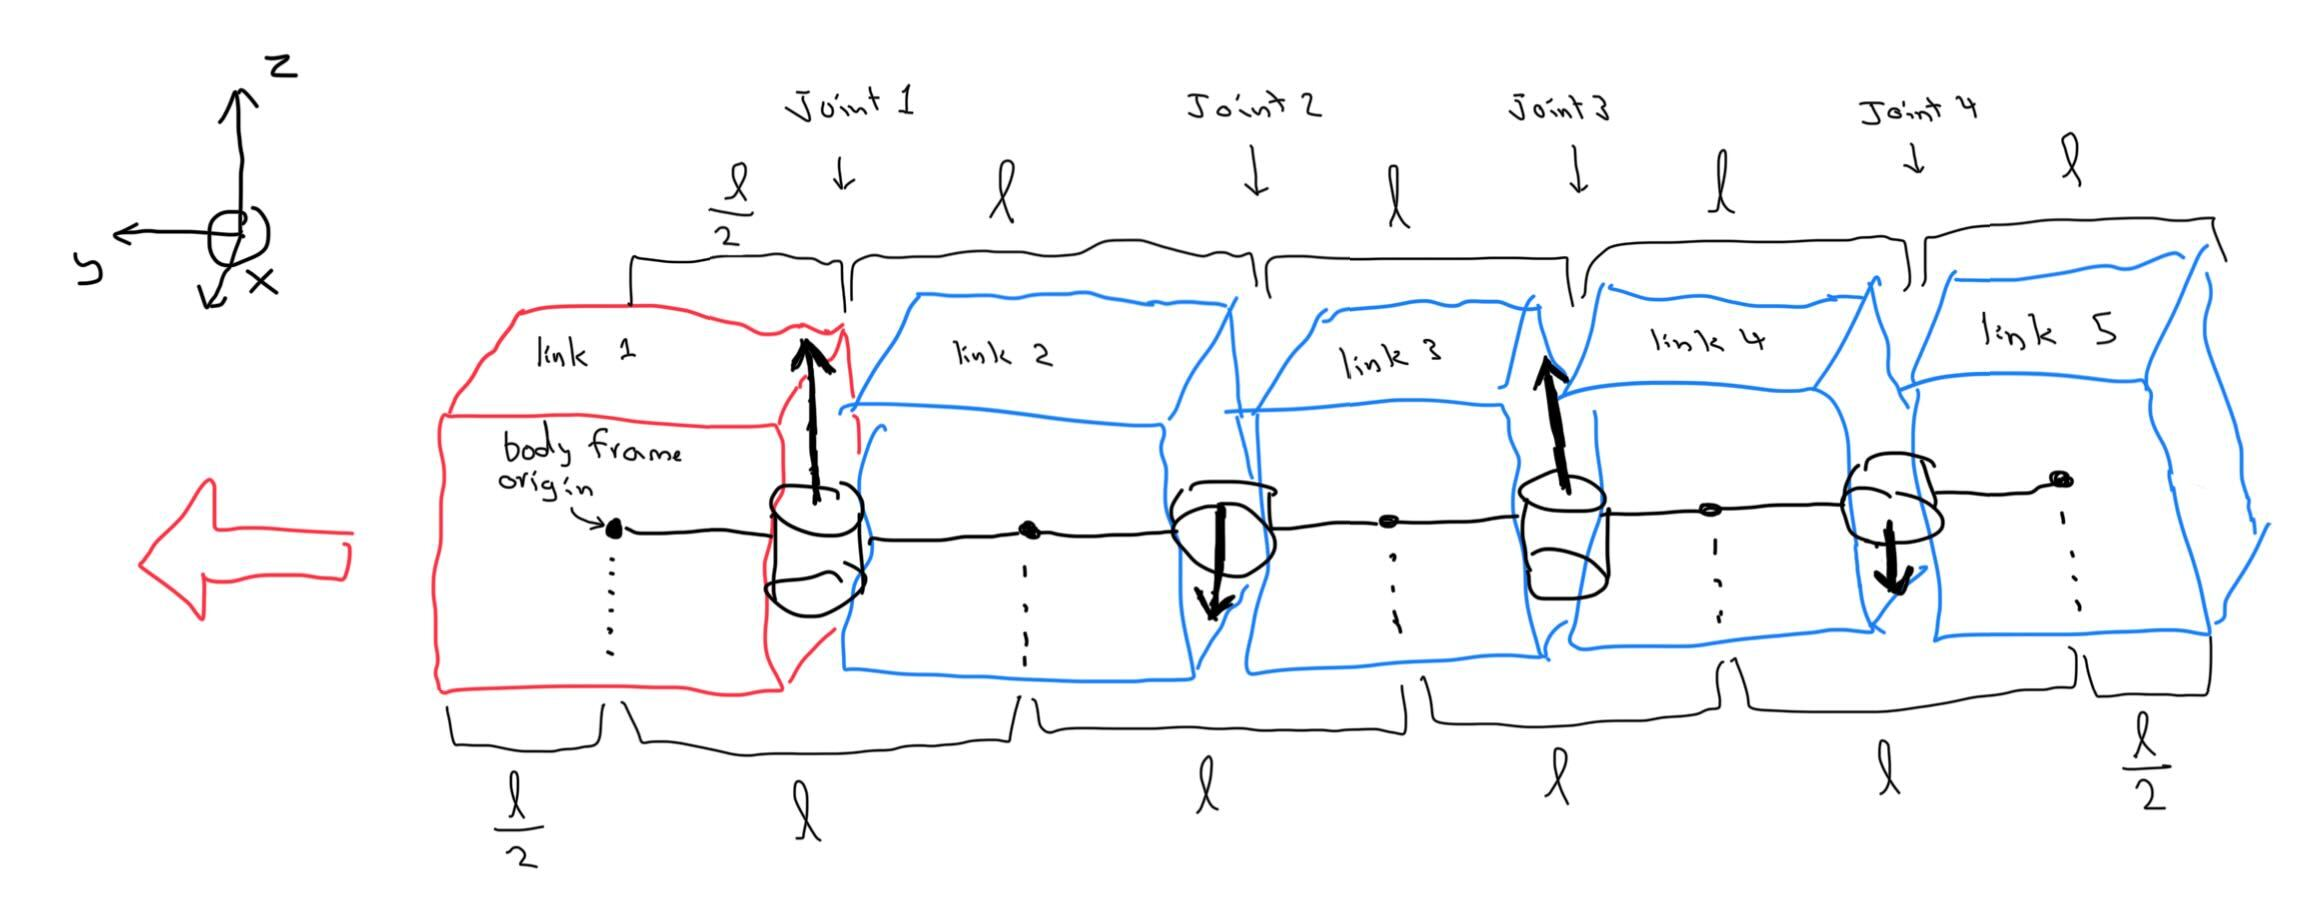
\includegraphics[width=1.2\textwidth]{snake_diagram.jpg}
    \caption{Example diagram of 4 joint snake robot.}
\end{figure}
\newpage 

\section{Forward Kinematics}
\begin{align*}
    g_{st}(\theta) &= e^{\hat{\xi}_1 \theta_1} e^{\hat{\xi}_2 \theta_2} \cdots e^{\hat{\xi}_N \theta_N} g_{st}(0) \\
    g_{si}(\theta) &= e^{\hat{\xi}_1 \theta_1} e^{\hat{\xi}_2 \theta_2} \cdots e^{\hat{\xi}_{i-1} \theta_{i-1}} g_{si}(0) \\
    \xi_i &= \begin{bmatrix}
        -\omega_i \times q_i \\
        \omega_i
    \end{bmatrix} \\
    \omega_i &= \begin{cases}
        \begin{bmatrix}
            1 & 0 & 0
        \end{bmatrix}^\top & i \text{ is even} \\
        \begin{bmatrix}
            0 & 0 & 1
        \end{bmatrix}^\top & i \text{ is odd}
    \end{cases} \\
    q_i &= \begin{bmatrix}
        0 \\ \frac{l}{2} + \sum_{j=1}^{i-1} l \\ 0
    \end{bmatrix} = \begin{bmatrix}
        0 \\ l(i - \frac{1}{2}) \\ 0
    \end{bmatrix} \\
    \xi_i &= \begin{cases}
        \begin{bmatrix}
            0 & 0 & -l(i-\frac{1}{2}) & 1 & 0 & 0
        \end{bmatrix}^\top & i \text{ is even} \\
        \begin{bmatrix}
            l(i-\frac{1}{2}) & 0 & 0 & 0 & 0 & 1
        \end{bmatrix}^\top & i \text{ is odd}
    \end{cases} \\
    g_{si}(0) &= \begin{bmatrix}
        1 & 0 & 0 & 0 \\
        0 & 1 & 0 & l(i-1) \\
        0 & 0 & 1 & 0 \\
        0 & 0 & 0 & 1
    \end{bmatrix}
\end{align*}

\section{Prediction Step}
\begin{align*}
    \mathbf{x}_k &= \begin{bmatrix}
        a_k \\ q_k \\ \omega_k \\ \theta_k \\ \dot{\theta}_k
    \end{bmatrix} \in \mathbb{R}^{10+2N} \\
    \mathbf{x}_k &= f(\mathbf{x}_{k-1}, \mathbf{u}_k) + \mathbf{w}_k \\
    &= \begin{bmatrix}
        e^{-\tau \Delta t} a_{k-1} \\
        \exp\left(-\frac{1}{2} \Psi(\omega_{k-1}) \Delta t\right) q_{k-1} \\
        \omega_{k-1} \\
        \theta_{k-1} + \dot{\theta}_{k-1} \Delta t \\
        (1 - \lambda) \dot{\theta}_{k-1} + \lambda \mathbf{u}_k
    \end{bmatrix} \\
    q_k &= \exp\left(-\frac{1}{2} \Psi(\omega_{k-1}) \Delta t\right) q_{k-1} \\
    &= \left(I \cos\left(\frac{\|\omega_{k-1} \Delta t\|}{2}\right) - \frac{1}{2} \begin{bmatrix}
        0 & -\omega^x \Delta t & \omega^y \Delta t & \omega^z \Delta t \\
        -\omega^x \Delta t & 0 & -\omega^z \Delta t & -\omega^y \Delta t \\
        -\omega^y \Delta t & \omega^z \Delta t & 0 & -\omega^x \Delta t \\
        -\omega^z \Delta t & -\omega^y \Delta t & \omega^x \Delta t & 0
    \end{bmatrix} \frac{\sin\left(\|\omega_{k-1} \Delta t\|\right)}{\|\omega_{k-1} \Delta t\|}\right) q_{k-1} \\
    F_k &= \pd{f}{\mathbf{x}_{k-1}} = \begin{bmatrix}
        e^{-\tau \Delta t} & 0 & 0 & 0 & 0 \\
        0 & \pd{q_k}{q_{k-1}} & \pd{q_k}{\omega_{k-1}} & 0 & 0 \\
        0 & 0 & 1 & 0 & 0 \\
        0 & 0 & 0 & 1 & \Delta t \\
        0 & 0 & 0 & 0 & 1
    \end{bmatrix} \\
    \pd{q_k}{q_{k-1}} &= TODO \\
    \pd{q_k}{\omega_{k-1}} &= TODO \\
\end{align*}

\section{Update Step}
\begin{align*}
    \mathbf{z}_k &= \begin{bmatrix}
        \phi_k \\ \alpha_k \\ \gamma_k
    \end{bmatrix} \in \mathbb{R}^{7N} \\
    \hat{\mathbf{z}}_k &= h(\mathbf{x}_k) \\
    &= \begin{bmatrix}
        \theta_k \\
        W_k^1 R_k g + \hat{a}^1_{\text{motion}} \\
        \vdots \\
        W_k^N R_k g + \hat{a}^N_{\text{motion}} \\
        \bar{\omega}^1 + (W_k^1)^\top \omega_k \\
        \vdots \\
        \bar{\omega}^N + (W_k^N)^\top \omega_k
    \end{bmatrix} \\
    W_k^i &= C_k g_{si}(\theta_k) \\
    \bar{\omega}^i &= \left(\frac{W_k^i(W_{k-1}^i)^{-1}}{\Delta t} - I\right)^\vee \\
    \hat{a}^i_{\text{motion}} &= TODO \\
    H_k &= \pd{h}{\mathbf{x}_k} = TODO \\
\end{align*}

\end{document}